% ACTIVITIES
% ------------------------------------------------------------ 
% A section discussing student organizations and extracurricular activities available to Berkeley students.

\vspace{1cm}
\addcontentsline{toc}{section}{Student Organizations and Activities}
\section*{Student Organizations and Activities}

The Nuclear Engineering graduate students are heavily involved in professional and student societies. 
Three organizations are organized within the department, described below. Additional professional societies include IEEE, INMM, ASME, AAAS, SWE, and numerous others.

\subsection*{The American Nuclear Society (UC Berkeley Student Chapter)}
 
\begin{wrapfigure}{r}{0.2\textwidth}
	\begin{center}
		\vspace{-1.0cm}
		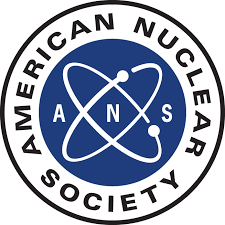
\includegraphics[width=3cm]{activities/ans_logo}
	\end{center}
\end{wrapfigure}

\textbf{The organization:} The American Nuclear Society (ANS) was established by a group of individuals who recognized the need to unify the professional activities within the diverse fields of nuclear science and technology. 
The core purpose of ANS is to promote the awareness and understanding of the application of nuclear science and technology.

The section’s primary goal is to provide a professional and social foundation for all nuclear engineering students (undergraduate and graduate).

\textbf{Activities:} Social events including bowling, scavenger hunts, happy hours, pub crawls, intramural sports teams, and movie nights. 
Each year a number of students travel to the ANS student conference, hosted by a different ANS student chapter. 
Members attend local ANS-Northern California meetings in San Francisco. 
Outreach activities include visiting K-12 schools, inviting students to visit our labs, and participating in campus wide events.

\vspace{1.0cm}
\begin{center}
	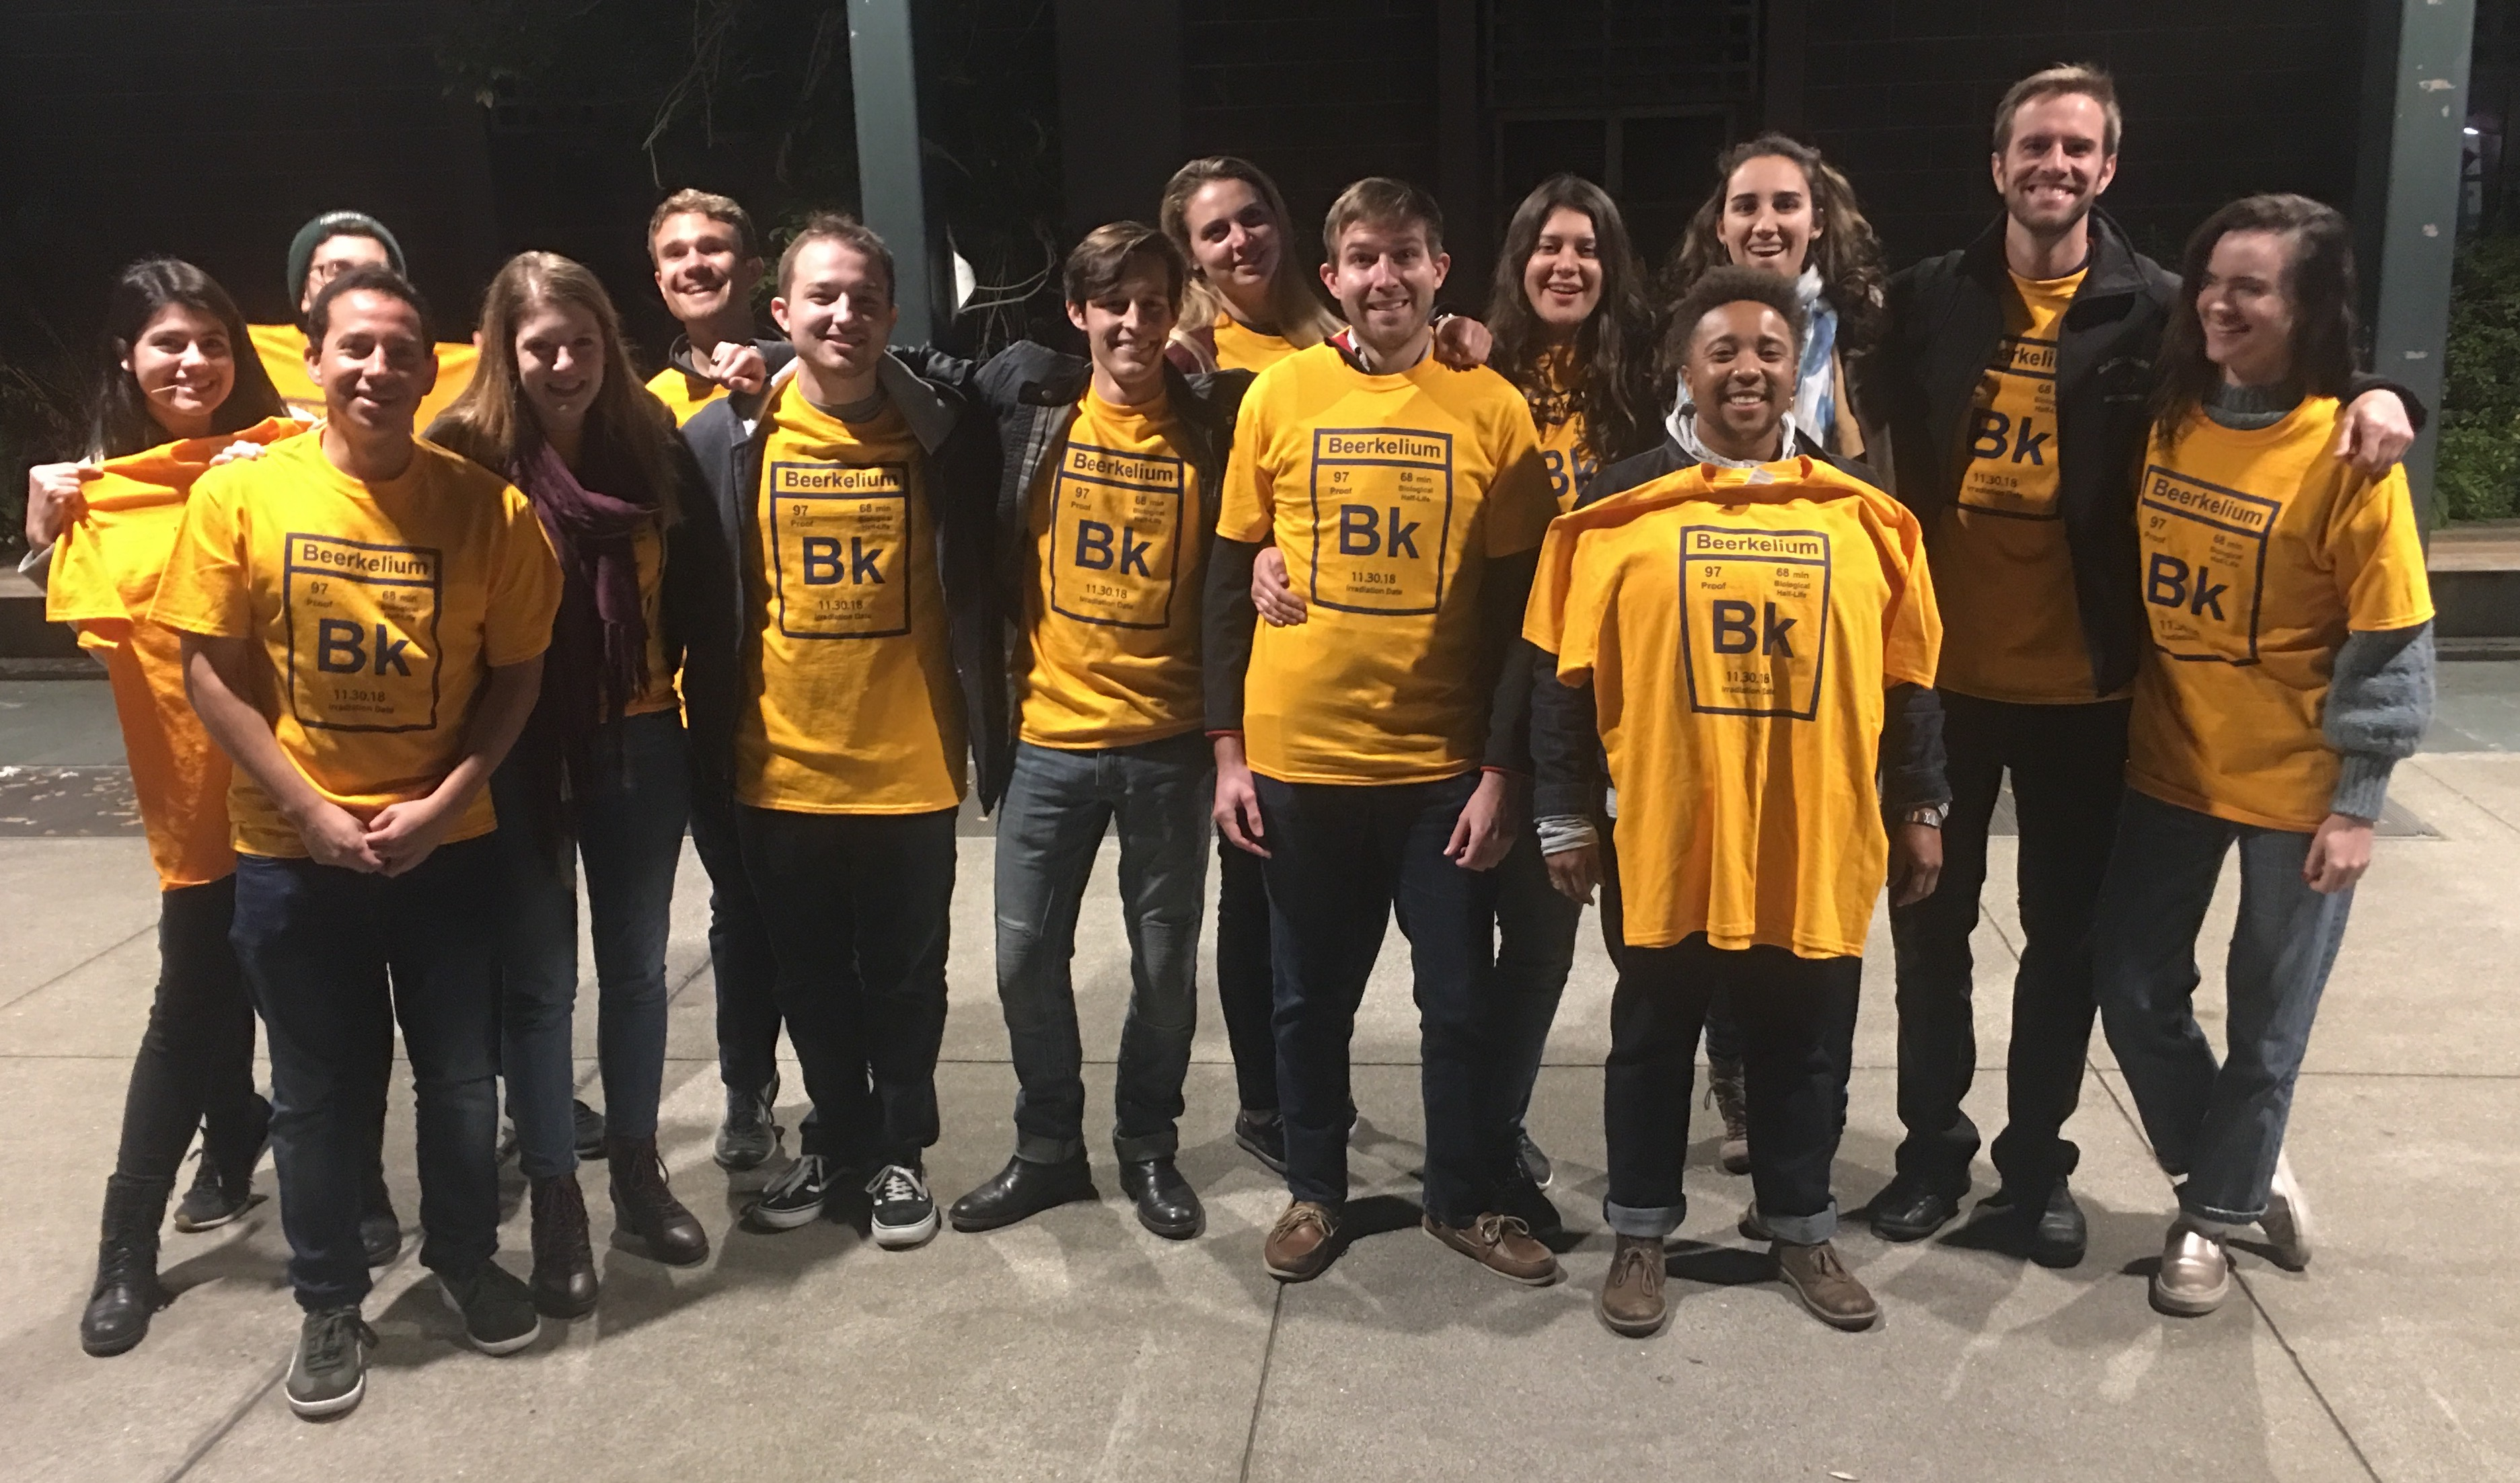
\includegraphics[width=15cm]{activities/ans_pub-crawl}
\end{center}

\clearpage
%\vspace{0.5cm}
\subsection*{Nuclear Outreach Group}
%% THIS NEEDS UPDATING!!!
The nuclear outreach group strives to shape public perception of nuclear energy through educational outreach and community involvement. 
The group celebrates Nuclear Science Week annually, hosting “scoutreach” events to introduce younger students to nuclear energy and setting up a booth at the East Bay Makers Fair. 
Currently, the group is working to introduce a ballot initiative for the 2018 election to amend Berkeley’s “nuclear free zone” designation to “nuclear weapons free.”

\vspace{0.5cm}
\begin{minipage}{0.5\textwidth}
	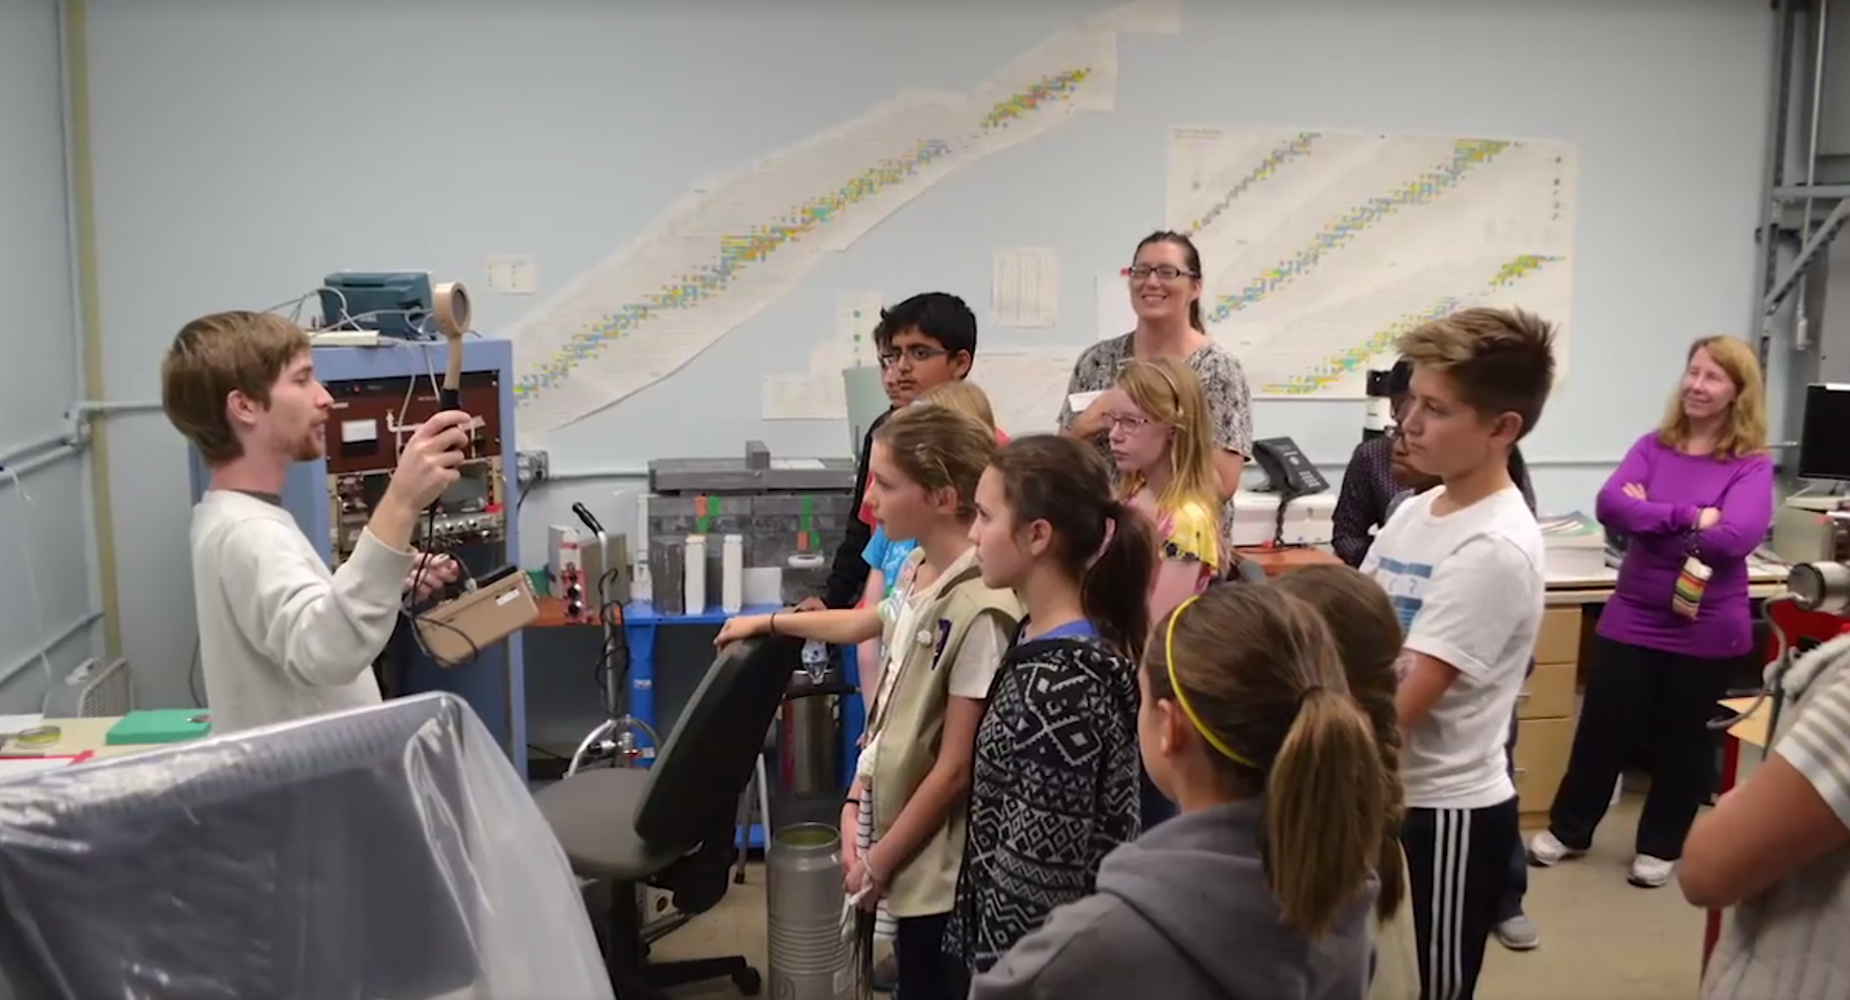
\includegraphics[width=\textwidth]{activities/neog_nsw-2017}
\end{minipage}
\begin{minipage}{0.5\textwidth}
	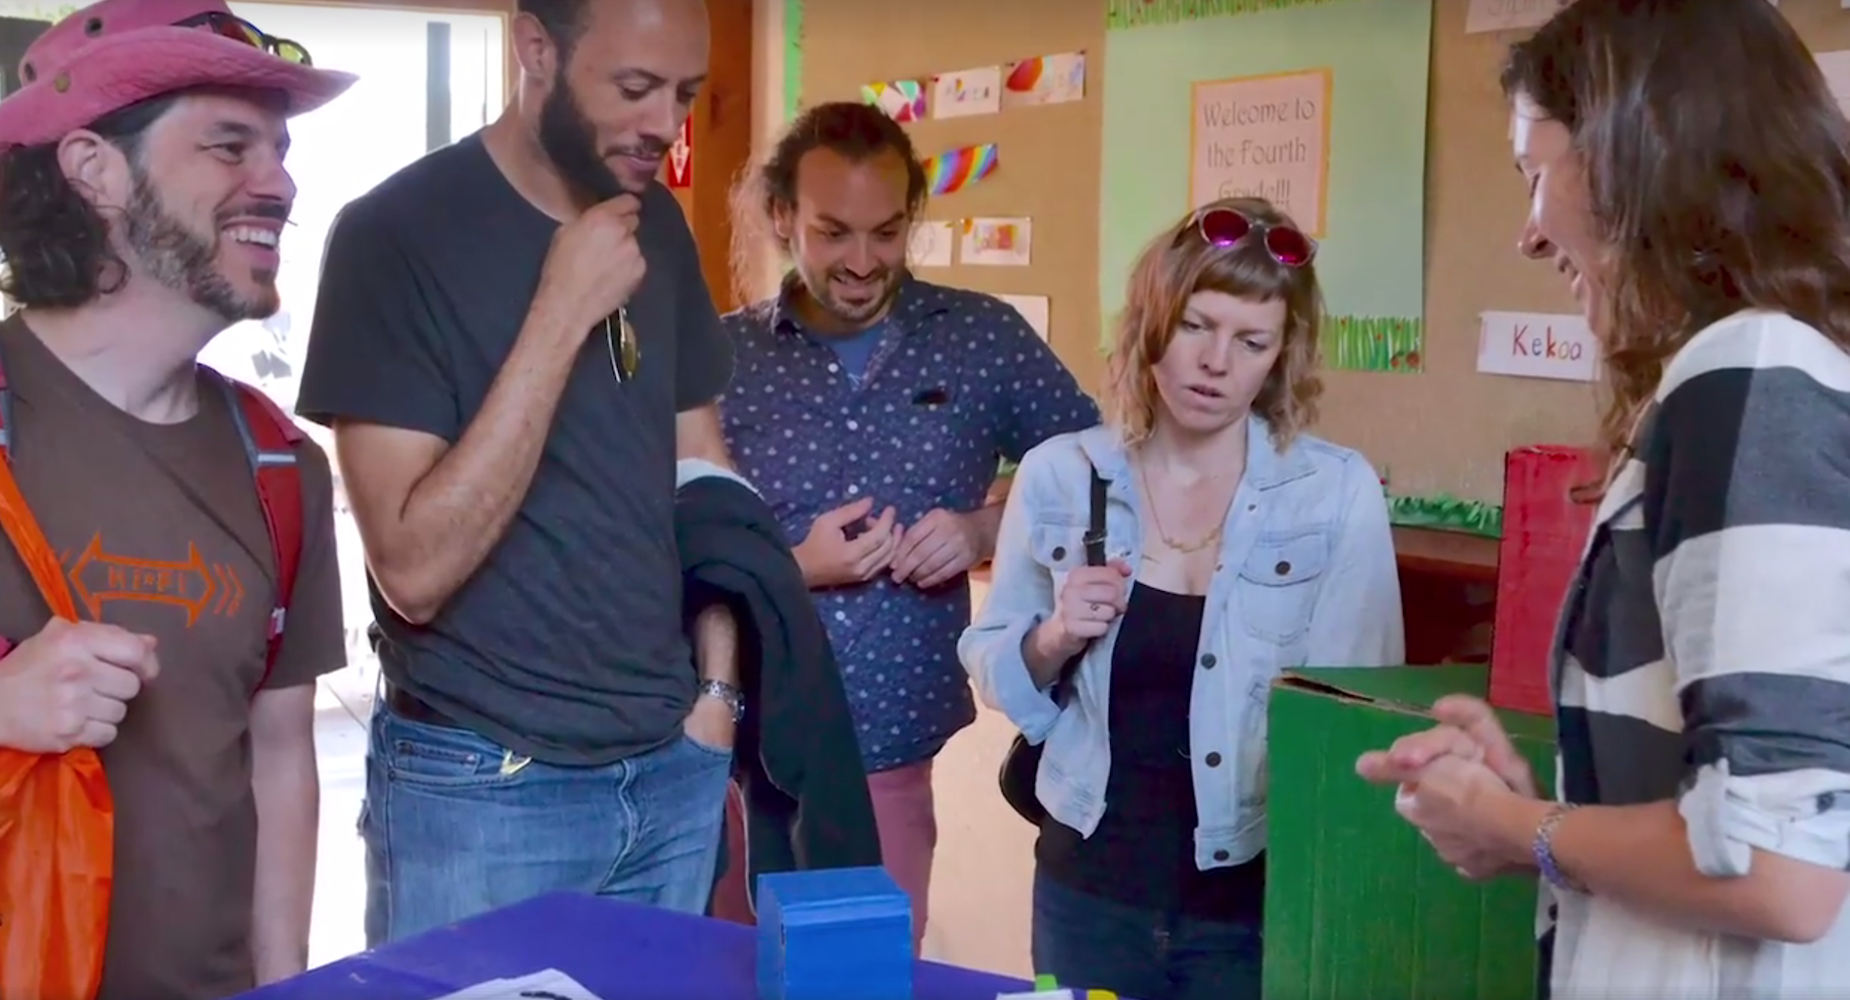
\includegraphics[width=\textwidth]{activities/neog_ebmf-2017}
\end{minipage}

Nuclear Outreach Group: (\textit{Left}) Chris Keckler teaches a scouting group about Geiger counters. (\textit{Right}) Maria Simanovskaia explains radioactive dose levels at the East Bay Maker Faire.

\vspace{1.5cm}

\begin{wrapfigure}{l}{0.4\textwidth}
	\begin{center}
		\vspace{-0.5cm}
		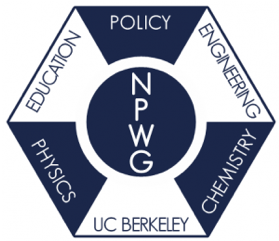
\includegraphics[width=5cm]{activities/npwg_logo}
	\end{center}
\end{wrapfigure}

\subsection*{Nuclear Policy Working Group}

The Nuclear Policy Working Group (NPWG) is a research-based educational programming effort that provides opportunities for students from a variety of fields to conduct multidisciplinary research on topics in nonproliferation and nuclear security. 
The NPWG has a three-fold mission: (1) to educate students on contemporary issues in nuclear security, (2) to foster collaboration across the technical and social science fields, and (3) to generate original policy-relevant publications. 

\clearpage
\subsection*{Recreational Sports}
Many students in the department stay active by playing intramural sports. UC Berkeley provides numerous options in this regard, with leagues of various degrees of skill and competitiveness. In the past few years, Berkeley Nuclear Engineering graduate students have fielded teams for soccer, futsal, volleyball, and softball. 

\vspace{0.5cm}
\begin{minipage}{0.98\textwidth}
	\begin{minipage}{0.5\textwidth}
		\begin{center}
			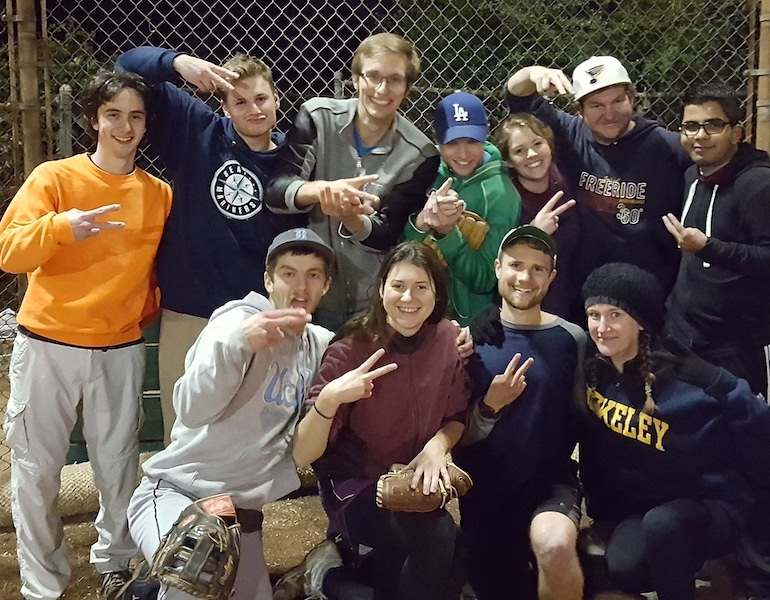
\includegraphics[height=6cm]{activities/eecs-softball_tsar-bomba}
		\end{center}
	\end{minipage}
	\begin{minipage}{0.5\textwidth}
		\begin{center}
			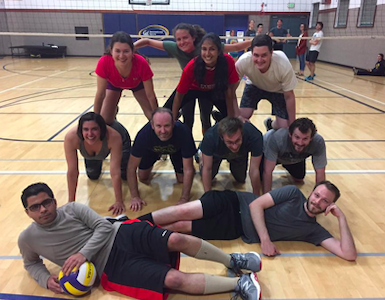
\includegraphics[height=6cm]{activities/rec-volleyball}
		\end{center}
	\end{minipage}
	\vspace{0.1cm}

	Sports: (\textit{Left}) The combined Nuclear Engineering/Physics softball team, Tsar Bomba. (\textit{Right}) The Nuclear Engineering intramural volleyball team.
\end{minipage}

\subsection*{NE Department Happy Hour}

The Nuclear Engineering Department has a tradition of enjoying a happy hour every Friday at 5:15 PM in the LaVal’s courtyard right near Etcheverry Hall. 
A great way to end the week, it almost always leads to other Friday night activities.

\vspace{0.25cm}
\begin{minipage}[t]{\textwidth}
	\begin{center}
		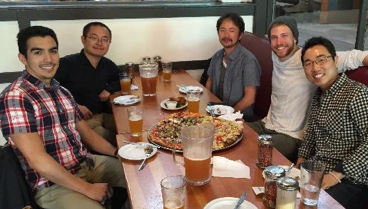
\includegraphics[height=6cm]{activities/happy-hour-01}
		\hspace{0.5cm}
		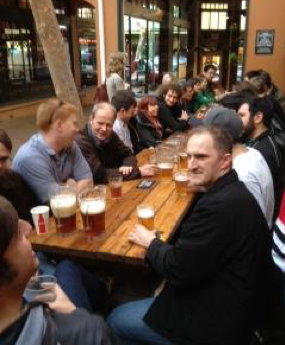
\includegraphics[height=6cm]{activities/happy-hour-02}
	\end{center}
\end{minipage}
